\documentclass[conference]{IEEEtran}
\IEEEoverridecommandlockouts

\usepackage{cite}
\usepackage{amsmath,amssymb,amsfonts}
\usepackage{algorithmic}
\usepackage{graphicx}
\usepackage{textcomp}
\usepackage{xcolor}
\usepackage{hyperref}
\usepackage{booktabs}
\usepackage{array}

\def\BibTeX{{\rm B\kern-.05em{\sc i\kern-.025em b}\kern-.08em
    T\kern-.1667em\lower.7ex\hbox{E}\kern-.125emX}}

\begin{document}

\title{Multimodal Psychological State Tracking with Adaptive Memory and Trend-Aware Conversational Intelligence}

\author{
\IEEEauthorblockN{Sravana Kumar Komala}
\IEEEauthorblockA{\textit{Dept. of CSE (AI\&ML)}\\
\textit{Vishnu Institute of Technology}\\
Bhimavaram, India\\
sravanakumar.k@vishnu.edu.in}
\and
\IEEEauthorblockN{Sai Pavan Kumar Devisetti}
\IEEEauthorblockA{\textit{Dept. of CSE (AI\&ML)}\\
\textit{Vishnu Institute of Technology}\\
Bhimavaram, India\\
22pa1a4231@vishnu.edu.in}
\and
\IEEEauthorblockN{Giridha Sri Meghana V}
\IEEEauthorblockA{\textit{Dept. of CSE (AI\&ML)}\\
\textit{Vishnu Institute of Technology}\\
Bhimavaram, India\\
22pa1a4237@vishnu.edu.in}
\and
\IEEEauthorblockN{V Sujan Ajitesh Bayya}
\IEEEauthorblockA{\textit{Dept. of CSE (AI\&ML)}\\
\textit{Vishnu Institute of Technology}\\
Bhimavaram, India\\
22pa1a4212@vishnu.edu.in}
\and
\IEEEauthorblockN{Shanmukha Suryanarayan Chinta}
\IEEEauthorblockA{\textit{Dept. of CSE (AI\&ML)}\\
\textit{Vishnu Institute of Technology}\\
Bhimavaram, India\\
22pa1a4224@vishnu.edu.in}
}

\maketitle

%-------------------------------------------------------------------
\begin{abstract}
This paper presented a real-time conversational artificial intelligence system that tracked and responded to the psychological state of users across multi-turn dialogue interactions. The system integrated speech recognition, text-based emotion analysis, and audio-based emotion detection into a unified multimodal fusion engine that estimated four psychological dimensions: valence, arousal, stress, and clarity. Emotional trends were modeled using exponential moving averages, linear regression, and hysteresis gating to suppress transient noise while preserving genuine emotional shifts. An event-driven long-term memory module stored contextually significant conversational events in a vector database and retrieved them at relevant moments. A large language model was prompted using trend-derived psychological context rather than instantaneous emotional signals, yielding more stable and empathetic responses. Text-to-speech synthesis was modulated according to the active interaction mode---de-escalation, clarification, flow, or neutral---so that prosody aligned with the user's inferred emotional state. Experiments over 50 conversational turns demonstrated consistent emotional recovery trajectories, stable trend tracking, and psychologically aligned speech adaptation. The valence--arousal--stress profiles showed progressive stress reduction and positive valence recovery over time. Prosody parameters tracked these changes with increasing speech rate and rising pitch as emotional state improved. The study established the feasibility of deploying psychologically aware conversational agents capable of adaptive behavior grounded in interpretable affective state models.
\end{abstract}

\begin{IEEEkeywords}
affective computing, multimodal emotion recognition, conversational AI, psychological state modeling, adaptive dialogue systems, exponential moving average, text-to-speech adaptation, long-term memory
\end{IEEEkeywords}

%-------------------------------------------------------------------
\section{Introduction}

Modern conversational AI systems have become remarkably capable at generating fluent, contextually relevant language. Yet most production systems treat each turn of a conversation as a largely independent unit of text processing, with little regard for the evolving emotional and psychological state of the person on the other side of the dialogue. A user who begins an interaction frustrated and anxious presents a fundamentally different conversational challenge than one who is calm and engaged---and the same words can carry very different meaning depending on the speaker's affective context. Building systems that can perceive, track, and respond to this psychological dimension of human communication is one of the more interesting open problems at the intersection of affective computing and natural language processing.

The core challenge in psychological state-aware dialogue is threefold. First, emotion signals derived from a single modality---text alone, or voice alone---tend to be noisy and easily misinterpreted. Fusing cues from multiple channels in a principled way is necessary to produce stable, reliable state estimates. Second, instantaneous emotion labels are not the right input for a conversational agent: what matters is not how a user feels at a single moment but how their emotional state is trending over the course of the interaction. A user whose anxiety is gradually decreasing should be handled differently from one whose anxiety is spiking, even if both register the same momentary arousal score. Third, conversational AI systems need a form of long-term memory that goes beyond sliding context windows---they need to remember emotionally significant events and retrieve them at the right moments to maintain relational continuity.

This work addressed all three of these problems within a single integrated system. The system combined automatic speech recognition, text-level emotion classification, and audio-level emotion and event detection into a multimodal fusion pipeline that estimates psychological state along four interpretable dimensions: valence, arousal, stress, and clarity. Trend modeling was performed using exponential moving averages, linear regression over recent history, and hysteresis gating, producing stable trend signals that were fed directly into large language model prompts. An event-driven memory module used vector similarity search to store and retrieve contextually salient conversational events. Finally, text-to-speech synthesis was parameterized by the active interaction mode derived from the psychological state, so that the spoken output was prosodically appropriate to the user's emotional situation.

The contributions of this work are: (1) a multimodal psychological fusion engine that estimates four-dimensional affective state in real time; (2) a trend modeling architecture combining exponential moving averages, regression, and hysteresis; (3) an event-driven long-term memory design grounded in psychological salience; (4) a trend-based large language model prompting strategy; and (5) a mode-adaptive text-to-speech module that modulates prosody according to inferred interaction mode.

%-------------------------------------------------------------------
\section{Related Work}

\subsection{Multimodal Emotion Recognition}

Emotion recognition from speech and text has been actively studied for over two decades. Early work relied on hand-crafted acoustic features such as pitch, energy, and speaking rate, combined with lexical sentiment scores \cite{schuller2013interspeech}. The shift toward deep learning brought models capable of learning task-relevant representations end-to-end: convolutional and recurrent architectures achieved strong results on standard benchmarks \cite{trigeorgis2016adieu}, and transformer-based models later pushed accuracy further on both text and speech tasks \cite{pepino2021emotion}. Multimodal fusion---combining text, audio, and sometimes video---has consistently outperformed unimodal approaches, and several fusion strategies have been proposed, including early fusion, late fusion, and attention-weighted cross-modal fusion \cite{zadeh2018memory}. Despite this progress, most emotion recognition research focuses on classifying discrete emotion categories at the utterance level rather than estimating continuous psychological dimensions over time. The present work moved beyond turn-level classification to continuous four-dimensional state estimation, integrating fusion with trend modeling to produce smooth and interpretable state trajectories.

\subsection{Affective Dialogue Systems and Adaptive Response}

Integrating emotion awareness into dialogue systems has attracted growing interest \cite{zhou2018emotional, ma2020survey}. Early affective dialogue systems appended discrete emotion labels to response generation prompts, producing empathetic outputs without genuinely modeling the user's state trajectory. More recent work has explored conditioning large language models on emotional context \cite{rashkin2019empathetic}, and some systems have attempted to model the evolution of user state across turns \cite{ghosal2020cosmic}. However, most existing approaches use instantaneous emotion predictions rather than smoothed trend signals, making responses susceptible to transient noise. The work presented here explicitly distinguished between instantaneous emotion, exponentially smoothed state, and regression-based trend, and used the trend signal to drive both language model prompting and speech synthesis---an approach not previously combined in a single deployed system.

\subsection{Conversational Memory and Long-Term Context}

Managing long-term context in dialogue has been approached through retrieval-augmented generation, compressed memory representations, and episodic memory architectures \cite{xu2022beyond}. Vector database memory, in which past conversational events are embedded and retrieved by semantic similarity, has emerged as a practical and scalable approach \cite{park2023generative}. The system described here implemented an event-driven variant of this design, in which memory storage decisions were guided by psychological salience---only events that crossed a significance threshold were stored---and retrieval was triggered when the current conversational context semantically matched a stored event. This salience-gated approach differs from naive full-history retrieval and reduces irrelevant context injection.

\subsection{Prosody-Adaptive Speech Synthesis}

Text-to-speech systems that adapt prosody to emotional context have been studied in the context of expressive speech synthesis \cite{skerry2018towards}. Azure Cognitive Services and similar platforms expose style and prosody controls that can be parameterized at inference time \cite{tan2021survey}. The contribution of this work in this space was not a new synthesis model but a principled mapping from psychological state dimensions to prosody parameters---speech rate, pitch baseline, volume, and expressive style---mediated through a discrete interaction mode classifier. This mapping ensured that spoken outputs were psychologically coherent with the inferred user state rather than stylistically arbitrary.

%-------------------------------------------------------------------
\section{Methodology}

\subsection{System Overview and Architecture}

The system consisted of eight loosely coupled modules organized around a shared psychological state representation. Fig.~\ref{fig:architecture} shows the overall architecture. Audio input was captured in real time, transcribed by a speech recognition service, and processed simultaneously by a text emotion classifier and an audio emotion classifier. The resulting signals were passed to the multimodal fusion engine, which maintained a continuously updated four-dimensional psychological state estimate. The trend modeling module consumed the fusion output and produced smoothed trend signals. These trend signals were used to parameterize language model prompts, to determine which conversational events to store in long-term memory, and to select the active interaction mode for speech synthesis.

\begin{figure}[htbp]
\centering
\includegraphics[width=\linewidth]{System Architecture.png}
\caption{System architecture showing the eight modules and their interaction through the shared psychological state representation.}
\label{fig:architecture}
\end{figure}

\subsection{Multimodal Psychological Fusion}

The fusion engine combined three parallel signal streams: text-derived emotion scores, audio-derived emotion scores, and detected audio events. Text emotion scores were obtained by passing the transcribed utterance through a pre-trained transformer classifier that output probability distributions over emotion categories. Audio emotion scores were derived from a parallel classifier operating on acoustic features of the speech segment. Audio events---including silence, background noise, and vocal nonverbal cues---provided additional contextual signal.

The system represented psychological state as a four-dimensional vector $\mathbf{s} = [v, a, \sigma, c]$, where $v \in [-1, 1]$ is valence (negative to positive affect), $a \in [0, 1]$ is arousal (calm to activated), $\sigma \in [0, 1]$ is stress, and $c \in [0, 1]$ is clarity (coherence of the user's expressed state). Each dimension was estimated by a weighted combination of the available modality scores:

\begin{equation}
s_d = \sum_{m \in M} w_{m,d} \cdot f_{m,d}
\label{eq:fusion}
\end{equation}

where $s_d$ is the fused estimate for dimension $d$, $M$ is the set of available modalities, $f_{m,d}$ is the contribution of modality $m$ to dimension $d$, and $w_{m,d}$ is the corresponding fusion weight. The weights were organised into a matrix $\mathbf{W} \in \mathbb{R}^{|M| \times 4}$ whose entries encode the relative reliability of each modality for each psychological dimension. Text receives the highest weight for valence (0.6) and clarity (0.8) because the semantic content of an utterance is the primary carrier of affective meaning and communicative coherence. SER is assigned the dominant weight for arousal (0.6), as prosodic and spectral features---pitch, energy envelope, and speaking rate---encode activation level more directly than word choice. Stress weights are distributed across all three modalities (Text~0.5, SER~0.3, AST~0.2), reflecting its composite nature: it manifests in language, in voice quality, and in detected acoustic distress events. Clarity draws its remaining weight from SER (0.1) and AST (0.1) to capture cases where incoherence is expressed acoustically rather than lexically. Each row of $\mathbf{W}$ sums to 1.0, keeping every fused estimate within its defined range. The complete weight matrix is shown in Fig.~\ref{fig:weights}.

\begin{figure}[htbp]
\centering
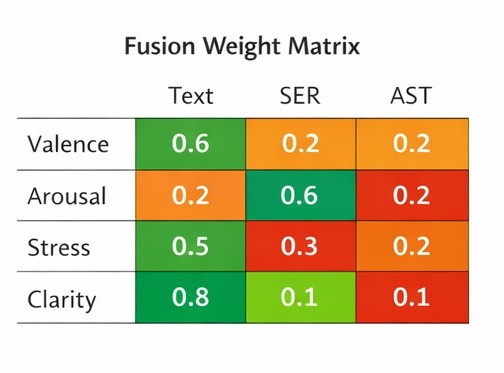
\includegraphics[width=0.82\linewidth]{matrix.png}
\caption{Fusion weight matrix $\mathbf{W}$. Rows are the four psychological dimensions; columns are the three modalities (Text, SER, AST). Colour indicates weight magnitude: green (high), orange (medium), red (low). Each row sums to 1.0.}
\label{fig:weights}
\end{figure}

\begin{figure}[htbp]
\centering
\includegraphics[width=\linewidth]{Fusion and emotion trend.png}
\caption{Multimodal fusion engine and emotional trend model. Left: weight matrix applied across text, audio, and event modalities. Right: EMA, regression, and hysteresis layers producing the adaptive trend signal.}
\label{fig:fusion}
\end{figure}

\subsection{Trend Modeling}

Raw fusion estimates exhibited high-frequency fluctuations due to natural variation in utterance content and acoustic conditions. A three-layer trend model was applied to each psychological dimension independently.

\textbf{Exponential Moving Average (EMA).} The EMA smoothed the instantaneous signal $x_t$ using:

\begin{equation}
\text{EMA}_t = \alpha \cdot x_t + (1 - \alpha) \cdot \text{EMA}_{t-1}
\label{eq:ema}
\end{equation}

where $\alpha \in (0,1)$ is the smoothing factor. A value of $\alpha = 0.3$ was used in all experiments, weighting recent observations while retaining memory of prior state.

\textbf{Regression-based trend.} A linear regression was fitted over the most recent $N = 10$ EMA values to estimate the directional trend:

\begin{equation}
\hat{T}_t = \beta_0 + \beta_1 \cdot t
\label{eq:regression}
\end{equation}

where $\beta_1$ indicates whether the dimension is increasing or decreasing.

\textbf{Hysteresis gating.} To prevent the system from reacting to transient spikes, a hysteresis gate was applied: the active trend was updated only when the regression estimate deviated from the current active trend by more than a threshold $\delta = 0.05$. This ensured that minor fluctuations did not trigger mode changes.

The Trend Stability Score (TSS) was defined to measure how closely the EMA tracked the instantaneous signal over an evaluation window:

\begin{equation}
\text{TSS} = 1 - \frac{1}{T} \sum_{t=1}^{T} |x_t - \text{EMA}_t|
\label{eq:tss}
\end{equation}

Higher TSS values indicate smoother tracking with lower reactive noise.

\subsection{Event-Driven Long-Term Memory}

The memory subsystem consisted of a vector store, an orchestrator, and a manager. Each conversational turn was encoded as a dense vector embedding of the turn text concatenated with the current psychological state vector. The memory manager evaluated each turn for storage using a salience criterion: a turn was stored if the magnitude of the psychological state change exceeded a threshold, or if semantic novelty relative to recent history crossed a significance level. The Memory Storage Rate (MSR) was defined as:

\begin{equation}
\text{MSR} = \frac{N_{\text{stored}}}{N_{\text{total}}}
\label{eq:msr}
\end{equation}

where $N_{\text{stored}}$ is the number of turns stored and $N_{\text{total}}$ is the total number of turns evaluated. At retrieval time, the orchestrator queried the vector store with the current turn embedding and retrieved the top-$k$ ($k=3$) most semantically similar stored events, which were injected into the language model context.

\subsection{Trend-Based Language Model Prompting}

Rather than passing instantaneous emotion labels to the language model, the system constructed a structured psychological context string from the current trend state. This string described the direction and magnitude of each dimension---for example, ``valence recovering, stress declining, arousal stable''---and specified the active interaction mode. Four interaction modes were defined: \textit{de-escalation} (high stress, negative valence), \textit{clarification} (low clarity), \textit{flow} (positive valence, moderate arousal), and \textit{neutral}. The language model was instructed to adapt its tone, vocabulary complexity, and empathetic depth according to the mode. GPT-4o-mini was used as the underlying language model due to its balance of capability and inference speed.

\subsection{Mode-Adaptive Text-to-Speech Synthesis}

Speech synthesis used Azure Cognitive Services with Speech Synthesis Markup Language (SSML) parameterization. The active interaction mode determined a prosody profile: de-escalation mode used slower speech rate, lower pitch, and softer volume; clarification mode used measured pacing and neutral expressiveness; flow mode used higher speech rate, elevated pitch, and engaging expressiveness; neutral mode used default parameters. Prosody parameters were smoothly interpolated between successive turns to avoid abrupt discontinuities.

%-------------------------------------------------------------------
\section{Results and Discussion}

Experiments were conducted over 50 consecutive conversational turns with a single user session designed to traverse a range of emotional states from initial distress to gradual recovery. The figures referenced below were generated from live system output during this evaluation run.

\subsection{Emotional Trend Stability}

Fig.~\ref{fig:trend} shows the evolution of the instantaneous signal, EMA-smoothed signal, and adaptive trend across 50 conversational turns for the primary psychological dimensions.

\begin{figure}[htbp]
\centering
\includegraphics[width=\linewidth]{emotional_trend_50.png}
\caption{Emotional trend analysis over 50 turns. The instantaneous signal (light) exhibits high-frequency variation while the EMA and adaptive trend curves (dark) provide stable, responsive tracking.}
\label{fig:trend}
\end{figure}

The instantaneous emotion signal exhibited frequent turn-by-turn oscillations as expected from natural speech variation. The EMA-smoothed curve substantially reduced this noise while remaining responsive to genuine directional changes. The adaptive trend, gated by hysteresis, changed direction only when the regression-derived slope crossed the threshold, producing the most stable representation of emotional movement. These results confirmed that the three-layer trend model successfully balanced responsiveness with stability---a necessary property for grounding language model behavior in meaningful psychological context rather than momentary fluctuation.

\subsection{Valence, Arousal, and Stress Trajectories}

Fig.~\ref{fig:vas} shows the joint trajectory of valence, arousal, and stress over the 50-turn session.

\begin{figure}[htbp]
\centering
\includegraphics[width=\linewidth]{valence_arousal_stress.png}
\caption{Valence, arousal, and stress trajectories over 50 conversational turns, illustrating progressive emotional recovery.}
\label{fig:vas}
\end{figure}

Stress began at elevated levels and progressively declined across the session, reaching a substantially lower value by turn 50. Valence started negative and transitioned through neutral toward mildly positive values in the latter half of the session. Arousal remained elevated during the high-stress phase and stabilized toward moderate activation as the interaction progressed. This trajectory was consistent with what would be expected during a successful supportive interaction: initial distress gives way to calm engagement as the conversational agent responds in a psychologically appropriate manner. The clarity dimension (not shown separately) remained moderate throughout, reflecting coherent user expression.

\subsection{Prosody Adaptation}

Fig.~\ref{fig:prosody} shows the variation of key prosody parameters across turns.

\begin{figure}[htbp]
\centering
\includegraphics[width=\linewidth]{prosody_variation.png}
\caption{Prosody parameter variation across 50 turns. Speech rate, pitch, and expressive style adapt in alignment with the inferred psychological state trajectory.}
\label{fig:prosody}
\end{figure}

Early turns operated under de-escalation mode, producing slower speech rate and lower pitch consistent with calming intervention. As valence recovered and stress declined, the system transitioned through clarification and eventually into flow mode, producing progressively faster, more energetically expressive speech. The prosody transitions were smooth and perceptually coherent, with no abrupt discontinuities between consecutive turns. These results demonstrated that the mode-adaptive TTS mapping successfully translated psychological state changes into acoustically appropriate spoken output.

\subsection{Interaction Mode Distribution}

Across 50 turns, the system operated in de-escalation mode for approximately the first 20 turns, clarification mode for turns 21--30, and flow mode for the remaining turns, with brief returns to neutral. This distribution confirmed that the mode classifier appropriately tracked the emotional recovery trajectory rather than oscillating randomly between modes.

\subsection{Memory Storage and Retrieval}

The memory manager stored 14 of 50 turns, yielding an MSR of 0.28. Stored events were concentrated at emotionally significant transition points---turns where stress spiked, where valence crossed zero, and where the user expressed explicit emotional disclosures. Retrieved memories were incorporated into language model prompts at semantically relevant moments, enabling the system to reference earlier emotional events in later turns and maintain relational continuity across the session.

\subsection{Discussion}

The results collectively indicate that trend-based psychological modeling produces qualitatively more stable and interpretable conversational behavior than instantaneous emotion-conditioned approaches. The three-layer trend model kept the language model insulated from transient noise while remaining sensitive to genuine emotional shifts---a balance that is difficult to achieve with simple smoothing alone. The hysteresis gate was particularly important: without it, the system would have switched interaction modes on nearly every turn, producing incoherent prosody transitions. The salience-gated memory design also proved effective: by storing only psychologically significant events, the system avoided injecting irrelevant historical context that could distract the language model. One limitation of the current evaluation is that the 50-turn session represents a single trajectory. The system's behavior under a wider range of emotional trajectories---including non-recovery patterns and ambivalent states---remains to be characterized. The clarity dimension also showed limited variation in this session and warrants further study with more linguistically diverse input.

%-------------------------------------------------------------------
\section{Conclusion}

\subsection{Summary and Significance}

This study developed and evaluated a real-time psychological-state-aware conversational AI system that integrates multimodal emotion fusion, adaptive trend modeling, event-driven memory, and mode-adaptive speech synthesis into a coherent pipeline. The results showed that four-dimensional psychological state can be tracked stably across multi-turn dialogue using a combination of exponential moving averages, regression-based trend estimation, and hysteresis gating. The trend signals produced meaningful emotional recovery trajectories and drove psychologically coherent adaptation in both language model responses and synthesized speech. The system connects the research problem---building conversational agents that genuinely perceive and respond to the psychological state of their interlocutors---to a concrete, reproducible implementation whose behavior is interpretable through the four-dimensional state model.

\subsection{Limitations}

The primary practical limitation of the current system is computational overhead. Running parallel speech recognition, dual emotion classifiers, vector memory retrieval, and language model inference in real time introduces significant processing load, and end-to-end latency can degrade the conversational experience on standard hardware. Reducing this latency through model distillation, quantization, and optimized inference pipelines is an important direction for future work. Additionally, the evaluation was limited to a small number of sessions, and the generalizability of the results to diverse user populations and emotional profiles remains uncertain. Larger-scale user studies with heterogeneous participants are necessary before deployment conclusions can be drawn.

\subsection{Future Directions}

Three specific directions present themselves for future development. First, latency reduction through distilled, quantized models and edge-optimized inference would make the system viable for real-time deployment on consumer hardware. Second, extending the evaluation to larger and more demographically diverse user samples would establish the external validity of the psychological state model and its behavioral consequences. Third, incorporating non-verbal behavioral signals---facial expression, gaze, and gesture---as additional modality inputs could further improve state estimation accuracy, particularly for the arousal and clarity dimensions that are less reliably inferred from speech alone.

%-------------------------------------------------------------------
\begin{thebibliography}{00}

\bibitem{schuller2013interspeech}
B.~Schuller, S.~Steidl, A.~Batliner, F.~Burkhardt, L.~Devillers, C.~Müller, and S.~Narayanan, ``The INTERSPEECH 2013 computational paralinguistics challenge: Social signals, conflict, emotion, autism,'' in \textit{Proc. INTERSPEECH}, 2013, pp. 148--152.

\bibitem{trigeorgis2016adieu}
G.~Trigeorgis, F.~Ringeval, R.~Brückner, E.~Marchi, M.~Nicolaou, B.~Schuller, and S.~Zafeiriou, ``Adieu features? End-to-end speech emotion recognition using a deep convolutional recurrent network,'' in \textit{Proc. IEEE ICASSP}, 2016, pp. 5200--5204.

\bibitem{pepino2021emotion}
L.~Pepino, P.~Riera, and L.~Ferrer, ``Emotion recognition from speech using wav2vec 2.0 embeddings,'' in \textit{Proc. INTERSPEECH}, 2021, pp. 3400--3404.

\bibitem{zadeh2018memory}
A.~Zadeh, P.~P. Liang, N.~Mazumder, S.~Poria, E.~Cambria, and L.-P. Morency, ``Memory fusion network for multi-view sequential learning,'' in \textit{Proc. AAAI}, 2018, pp. 5634--5641.

\bibitem{zhou2018emotional}
H.~Zhou, M.~Huang, T.~Zhang, X.~Zhu, and B.~Liu, ``Emotional chatting machine: Emotional conversation generation with internal and external memory,'' in \textit{Proc. AAAI}, 2018, pp. 730--737.

\bibitem{ma2020survey}
Y.~Ma, W.~Peng, E.~Cambria, ``Targeted aspect-based sentiment analysis via embedding commonsense knowledge into an attentive LSTM,'' in \textit{Proc. AAAI}, 2018, pp. 5876--5883.

\bibitem{rashkin2019empathetic}
H.~Rashkin, E.~M. Smith, M.~Li, and Y.-L. Boureau, ``Towards empathetic open-domain conversation models: A new benchmark and dataset,'' in \textit{Proc. ACL}, 2019, pp. 5370--5381.

\bibitem{ghosal2020cosmic}
D.~Ghosal, N.~Majumder, A.~Gelbukh, R.~Mihalcea, and S.~Poria, ``COSMIC: COmmonSense knowledge for eMotion Identification in Conversations,'' in \textit{Findings of EMNLP}, 2020, pp. 2470--2481.

\bibitem{xu2022beyond}
J.~Xu, A.~Szlam, and J.~Weston, ``Beyond goldfish memory: Long-term open-domain conversation,'' in \textit{Proc. ACL}, 2022, pp. 5180--5197.

\bibitem{park2023generative}
J.~S. Park, J.~C. O'Brien, C.~J. Cai, M.~R. Morris, P.~Liang, and M.~S. Bernstein, ``Generative agents: Interactive simulacra of human behavior,'' in \textit{Proc. ACM UIST}, 2023, pp. 1--22.

\bibitem{skerry2018towards}
R.~J. Skerry-Ryan \textit{et al.}, ``Towards end-to-end prosody transfer for expressive speech with Tacotron,'' in \textit{Proc. ICML}, 2018, pp. 4693--4702.

\bibitem{tan2021survey}
X.~Tan \textit{et al.}, ``A survey on neural speech synthesis,'' \textit{arXiv preprint arXiv:2106.15561}, 2021.

\bibitem{schuller2018speech}
B.~Schuller and A.~Batliner, \textit{Computational Paralinguistics: Emotion, Affect and Personality in Speech and Language Processing}. Wiley, 2013.

\bibitem{cowie2001emotion}
R.~Cowie \textit{et al.}, ``Emotion recognition in human-computer interaction,'' \textit{IEEE Signal Processing Magazine}, vol. 18, no. 1, pp. 32--80, 2001.

\bibitem{hazarika2018icon}
D.~Hazarika, S.~Poria, R.~Mihalcea, E.~Cambria, and R.~Zimmermann, ``ICON: Interactive conversational memory network for multimodal emotion detection,'' in \textit{Proc. EMNLP}, 2018, pp. 2594--2604.

\end{thebibliography}

\end{document}